\errorcontextlines=5

%%%

\documentclass[
%handout,
]{beamer}

\usepackage{ifluatex}
\ifluatex\else\errmessage{This document requires LuaLaTeX}\fi

\usepackage{etex,etoolbox}
\usepackage{fontspec}
\usepackage[ngerman]{babel}
\usepackage{csquotes}
\usepackage{array}
\usepackage{wrapfig}
\usepackage{booktabs}
\usepackage{ccicons}
\usepackage{calc}

\usepackage{tikz}
\usetikzlibrary{arrows,intersections,calc,through,%
  external,positioning,automata,datavisualization,%
  datavisualization.formats.functions}

\usepackage{luacode}
\usepackage{pgfplots}
\usepackage{manfnt}

%%% title and such

\title{Wissenschaftliches Arbeiten mit \LaTeX}
\author{\texorpdfstring{Felix Hilsky\\basierend auf einem Kurs von\\Daniel Borchmann,\\Tom Hanika und \\Max Marx}{Felix Hilsky basierend auf einem Kurs von Daniel Borchmann, Tom Hanika und Max Marx}}
\titlegraphic{\ccLogo \ccAttribution \ccShareAlike}

%%% theme

\usepackage{tikz}
\usetikzlibrary{shapes.multipart}
\usetheme{CambridgeUS}
\setbeamertemplate{blocks}[rounded][shadow=false]
\setbeamertemplate{items}{\raisebox{0.3ex}{%
    \tikz[scale=0.13] \draw[fill] (0,0) -- (0,1) -- (0.9,0.5) -- cycle;}}
\usetikzlibrary{arrows}
\tikzset{>={stealth'[sep]}}
\setbeamertemplate{navigation symbols}{}
\setbeamertemplate{footline}{}
\setlength{\abovedisplayskip}{0pt}
\setbeamerfont{title}{series=\bfseries}
\defbeamertemplate{block alerted begin}{bends}{%
  \begin{columns}
    \begin{column}{0.05\linewidth}
      \dbend
    \end{column}
    \begin{column}{0.95\linewidth}
      \vskip.75ex\usebeamercolor[fg]{block title
        alerted}\insertblocktitle{}
      \vskip.1em
      \usebeamercolor[fg]{normal text}
}
\defbeamertemplate{block alerted end}{bends}{%
    \end{column}
  \end{columns}
}
%%%

\mode<handout>{
  \usepackage{pgfpages}
  \pgfpagesuselayout{2 on 1}[a4paper,border shrink=5mm]
}

%%% lecture organization

\usepackage{xparse}
\DeclareDocumentCommand \Lecture { m m }{%
  \lecture{#1}{#2}
  \part{#1}
  \include{#2}
}

\AtBeginSection{
  \setbeamertemplate{blocks}[rounded][shadow=true]
  \begin{frame}[plain]
    \begin{block}{}
      \begin{center}
        \textcolor{darkred}{\textbf{\Large \strut\smash{\insertpart}}}\\[1ex]
        \textcolor{blue!70!black}{\strut\smash{\insertsection}}
      \end{center}
    \end{block}
  \end{frame}
  \setbeamertemplate{blocks}[rounded][shadow=false]
  \setbeamertemplate{block alerted begin}[bends]
  \setbeamertemplate{block alerted end}[bends]
}

%%% misc

\newcommand{\GNULinux}{GNU\lower-0.25ex\hbox{/}Linux}
\newcommand{\TikZ}{Ti\emph{k}Z}

\usepackage{listings}

\lstset{language=[LaTeX]TeX, basicstyle=\ttfamily,
  keywordstyle={\color{blue}\bfseries}, frame=tb, extendedchars=true, literate=%
  {ä}{{\"a}}1 {ö}{{\"o}}1, escapeinside={(*@}{@*)}, mathescape=true,
  basewidth=0.5em, keywordstyle={\color{blue}},
  morekeywords={[0]includegraphics,rotatebox,scalebox,resizebox,providecommand,
    subsection,subsubsection,paragraph,subparagraph,part,chapter,tableofcontents,
    mathring,text,mathbb,printindex,addbibresource,printbibliography,subtitle,
    institute,titlegraphic,subject,keywords,draw,path,color,textcolor,toprule,
    midrule,bottomrule,maketitle,setlength,enquote,listoffigures,listoftables,
    theoremstyle,theoremheaderfont,theorembodyfont,newblock,parencite,footcite,
    autocite,bibitem,middle,tikzset,usetikzlibrary,coordinate,node,foreach,
    datavisualization,varepsilon,autocite,bibitem,DeclareRobustCommand,
    DeclareDocumentCommand,IfBooleanTF,bye,frametitle,setbeamertemplate,pause,
    onslide,uncover,visible,invisible,only,alt,temporal,alert,AtBeginSection,
    usetheme,setbeamerfont,tikz,includeonlyframes,mode,pgfpagesuselayout,RequirePackage,
  },
}

\AtBeginDocument{\frame[plain]{\maketitle}}

%%% end of preamble
\subtitle{Nummerierung, Referenzierung, Bibliographie}
\date{2017-05-16}

\begin{document}

\section{Referenzieren}

\begin{frame}[fragile]
  \frametitle{Verweise im Dokument}

  \onslide<+->

  \LaTeX\ erlaubt die automatische Erstellung von Verweisen innerhalb des Dokuments

  \begin{itemize}
  \item<+-> mit dem Befehl \lstinline!\label{label-name}! wird ein \emph{Label} im Dokument
    gesetzt
  \item<+-> mit dem Befehl \lstinline!\ref{label-name}! wird auf dieses Label verwiesen
  \end{itemize}

  \onslide<+->

\begin{lstlisting}
\section{Einführung}
\label{sec:introduction}

Das Problem, welches wir behandeln wollen, ist wichtig!

\section{Das Problem}

Siehe Abschnitt~\ref{sec:introduction}!
\end{lstlisting}

  \onslide<+->

  \emph{Wichtig}: Zweimaliges Übersetzen notwendig! (Machen viele Editoren automatisch.)
  % beim ersten Mal werden die Informationen für die Label gesammelt. Beim zweiten Mal bei den Referenzierungen eingesetzt.
  % Demonstrieren: beim ersten Mal entstehen ??. -> in Übung
  % Demonstrieren: Zeilen in aux-Datei -> in Übung

\end{frame}

\begin{frame}[fragile]
  \frametitle{Platzierung von Labeln}

  \onslide<+->

  % Die Formatierung von \lstinline!\ref{label-name}! hängt von dem Verweis ab.
  % was wollte Daniel uns damit sagen?
  Faustregel: alles, was eine Nummer hat, kann mit einem Label versehen werden.

  \onslide<+->
% an Konvention kat:name erinnern
\begin{lstlisting}
\section{Abschnitt} \label{sec:section} % Verweis auf Abschnittsnummer
\begin{enumerate}
\item\label{item:eintrag} Eintrag % Verweis auf Einzelpunkt
\end{enumerate}
\begin{figure}
  $\dots$                 % Verweis auf Abbildung
  \caption{\label{fig:mein Bild} Bildunterschrift}
\end{figure}
\begin{equation}
  \int a dx = b \label{eq:int} % Verweis auf Formel
\end{equation} % bei align kann auf jede Zeile verwiesen werden
\end{lstlisting}

  \onslide<+->

  Verweis auf die Seitenzahl mit \lstinline!\pageref{label-name}!.

\end{frame}

\begin{frame}[fragile]
  \frametitle{Nützliche Pakete}

  \onslide<+->

  Es gibt einige nützliche Pakete, die Verweise besser formatieren können

  \begin{itemize}
    \item<+-> \lstinline!hyperref! macht aus Verweisen klickbare Links (und noch viel mehr) $\to$ fast immer nutzen
    \item<+-> \lstinline!amsmath! gibt den Befehl \lstinline!\eqref{eq:ref}!, der die Klammern um den Verweis setzt: %\eqref{eq:int}.
    \item<+-> \lstinline!ntheorem! gibt den Befehl \lstinline!\thref{thm:main-theorem}!,
      welcher automatisch den Typ der Aussage hinzufügt (Satz~5.1, Lemma~5.1, Bemerkung~5.1,
      \dots)
    \item<+-> \lstinline!cleveref! gibt \lstinline!\cref! und weitere Befehle, welche
      automatisch den Typ der Referenz hinzufügen
    \item<+-> \lstinline!varioref! gibt \lstinline!\vref!, \lstinline!\vpageref!, und
      weitere, welche intelligente Formatierungen abhängig vom Abstand zwischen Referenz und
      Verweis erlauben
  \end{itemize}

\end{frame}

\section{Literaturverzeichnisse}

\begin{frame}
  \frametitle{Ziel}

  \begin{center}
  %\item<+-> 
  Erstellung von Literaturverzeichnissen in \LaTeX mit Bib\LaTeX
  % \item<+-> Automatische Erstellung mittels Bib\TeX
  % \item<+-> Anpassung von Zitier- und Verzeichnisstilen mit Bib\LaTeX
  \end{center}

\end{frame}

\section{Manuelle Erstellung}

\begin{frame}[fragile]
  \frametitle{Es geht auch manuell mit \LaTeX}
  % \onslide<+->

  \begin{itemize}
    \item<+-> Anlegen eines Literaturverzeichnisses innerhalb der Umgebung \lstinline!thebibliography!
    \item<+-> Zitierne im Text mit \lstinline!\cite{Key}!
  \end{itemize}
  % sagen:
  %   \item<+-> Aufwendig
  %   \begin{itemize}
  %   \item<+-> Jede Referenz muss einzeln formatiert werden
  %   \item<+-> Verwendete Referenzen müssen manuell zusammengestellt werden
  %   \item<+-> Manuelle Sortierung
  %   \end{itemize}
  % \item<+-> Unflexibel
  %   \begin{itemize}
  %   \item<+-> Änderung der Verzeichnis-Formatierung?
  %   \item<+-> Änderung der Zitat-Formatierung?
  %   \item<+-> Hinzufügen und Löschen von Quellen?
  %   \end{itemize}
  % \item<+-> Fehleranfällig
  % \end{itemize}
\end{frame}

\section{Bib\TeX}

\begin{frame}[fragile]
  \frametitle{Automatisch mit BibTex}
  \onslide<+->

  \begin{itemize} %[Vorteile]
    \item<+-> Automatische Erstellung von \lstinline|thebibliography|-Umgebungen
    \item<+-> Automatische Sortierung
    % \item<+-> Automatische Formatierung nach vordefinierten Stilen
    % \item<+-> Verwendung von separaten Paketen zur Anpassung der Zitat-Stile.
  \end{itemize}

  \onslide<+->

  Autoren: Leslie Lamport, Oren Patashnik, 1985

  %nicht automatisch veraltet, hat aber Schwächen
  \begin{itemize}
    \item<+-> Bib\TeX\ bestimmt nur die Formatierung des
      Literaturverzeichnisses, nicht der Quellenverweise
    % \begin{itemize}
    %   \item<+-> Widerspricht dem Prinzip der Trennung von Inhalt und Form
    % \end{itemize}
    \item<+-> Anpassung von Bib\TeX-Stilen \emph{sehr aufwendig} (eigene
      Programmiersprache) %, in Postfix-Notation)
    \item<+-> Unterstützung für UTF-8 fehlt% (kleine Abhilfe: \texttt{bibtex8}) % gerade bei Autorennamen kommen ungewöhnliche Zeichen vor
  \end{itemize}
  \onslide<+->
  \centerline{$\implies$ Nutze Bib\LaTeX}
\end{frame}

\begin{frame}[fragile]
  \frametitle{Bib\TeX-\enquote{Datenbanken}}
  % \onslide<+->

  \begin{itemize}
  \item<+-> Zur Verwendung von Bib\LaTeX müssen die Literaturquellen in
    einer \enquote{Bib\LaTeX-Datenbank} abgelegt werden.
  \item<+-> Dies ist eine Textdatei in einem bestimmten Format\onslide<+->%
\begin{lstlisting}
@article{Key,
  title     = {Was soll das alles?},
  author    = {John Doe and Otto Normalverbraucher},
  journal   = {Zeitschrift der Zukunft},
  year      = {2015},
  publisher = {Fantasy Press},
}
\end{lstlisting}
  \item<+-> Formate \verb|@article|, \verb|@book|, \verb|@proceedings|,
    \verb|@inproceedings|, \verb|@misc|, \dots
  \item<+-> siehe Dokumentation von \lstinline|biblatex|
  \end{itemize}

\end{frame}

\begin{frame}[fragile]
  \frametitle{Aufruf}
  % \onslide<+->

  \begin{itemize}
  \item<+-> In der \LaTeX-Datei in der Präambel:
\begin{lstlisting}
\usepackage[backend=biber]{biblatex}  % default: bibtex
\addbibresource{quellen1.bib}           % statt biber, veraltetz
\end{lstlisting}
  \item<+-> In der \LaTeX-Datei zum Einfügen der Bibliographie:
\begin{lstlisting}
\printbibliography
\end{lstlisting}
  \item<+-> In der \LaTeX-Datei zum Einfügen eines Verweises:
\begin{lstlisting}
\autocite{key}
\end{lstlisting}
\end{itemize}
\end{frame}

\begin{frame}[fragile]
  \frametitle{Übersetzung}
  \begin{itemize}
    \item<+-> Aufruf \LaTeX, dann biber, dann \LaTeX\ (zwei Mal)
    \onslide<+->
\begin{verbatim}
$ pdflatex myfile.tex
$ biber myfile          # ohne Dateiendung! 
$ pdflatex myfile.tex
$ pdflatex myfile.tex
\end{verbatim}
    \begin{itemize}
    \item<+-> Erster Aufruf extrahiert alle Quellen aus dem Dokument
    \item<+-> Aufruf von Bib\TeX\ formatiert und sortiert die
      verwendeten Referenzen
    \item<+-> Nächster Aufruf von \LaTeX\ fügt Literaturverzeichnis ein
    \item<+-> Letzter Aufruf von \LaTeX\ fügt Quellenzitate ein
    \end{itemize}
  \item<+-> Wird meist automatisch von der Entwicklungsumgebung gemacht
  \end{itemize}

\end{frame}

\begin{frame}[fragile]
  \frametitle{Woher Bib\TeX-Einträge bekommen?}

  \centering

  \only<2>{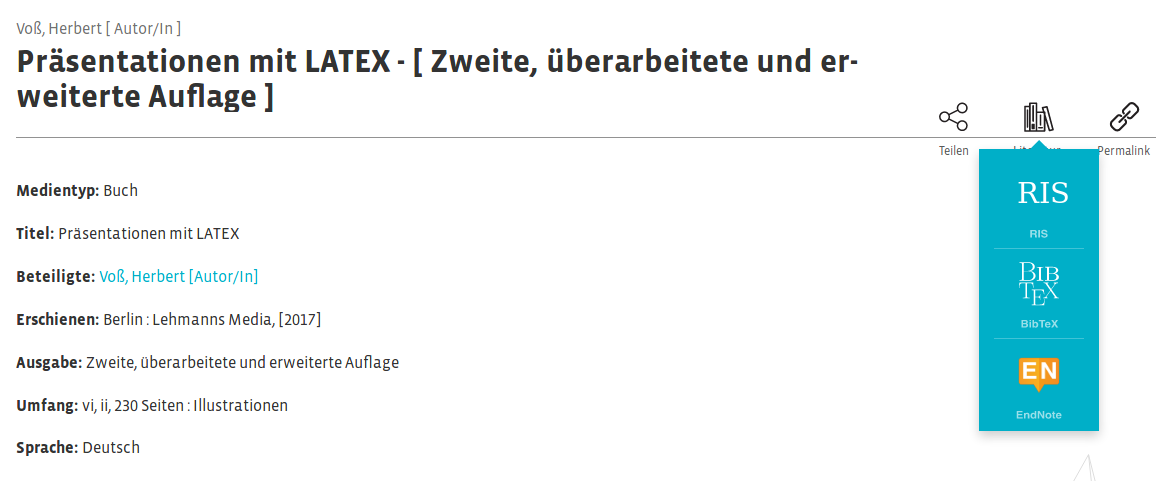
\includegraphics[height=\textheight, width=\textwidth, keepaspectratio]{pics/bibresourceslub.png}}
  \only<3>{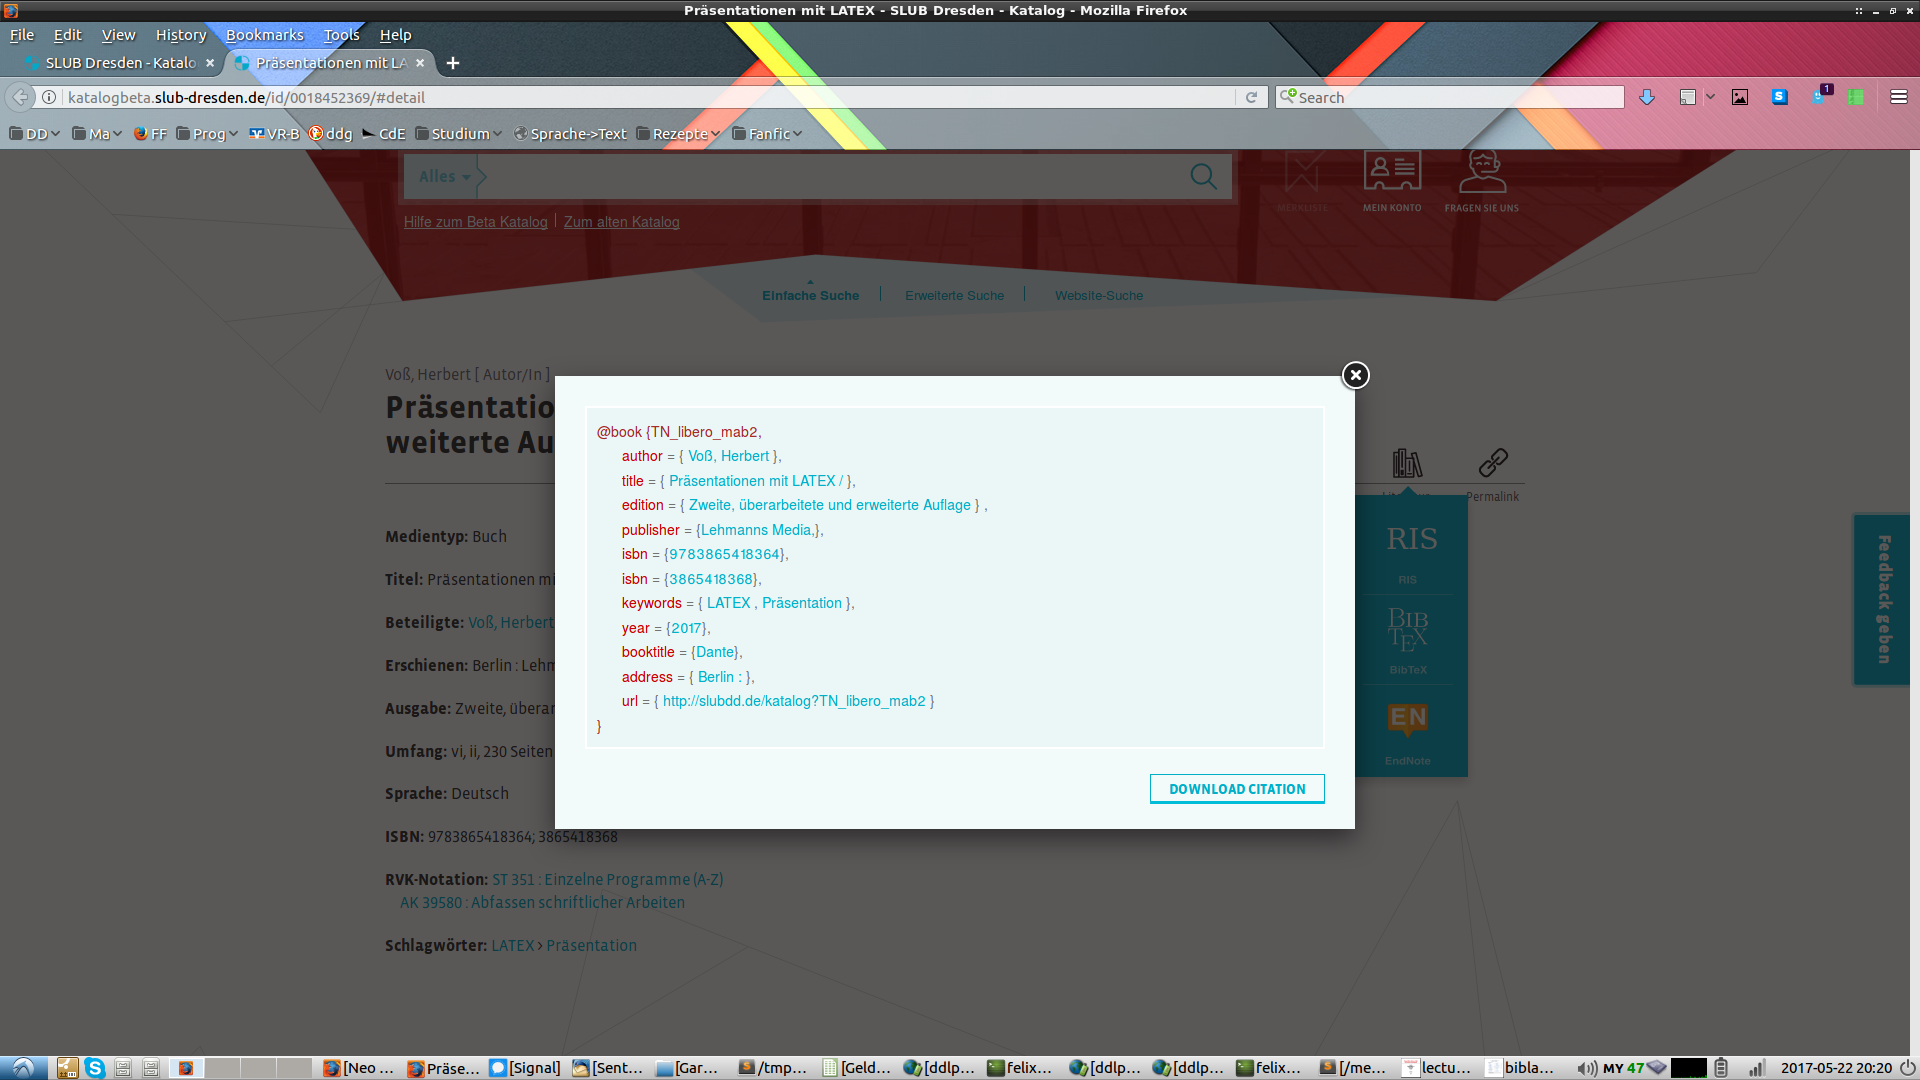
\includegraphics[height=\textheight, width=\textwidth, keepaspectratio]{pics/bibresourceslubatbook.png}}

\end{frame}

\begin{frame}[fragile]
  \frametitle{Stile}
  \begin{itemize}
    \item Es gibt viele ($\geq 295$) Bib\TeX-Stile.
    \item Meist durch andere (Institut, Zeitschrift, etc.) vorgegeben.
    \item Angegeben in der Präambel
\begin{lstlisting}
\usepackage[style=numeric-comp,  % Alternativen:
            backend=biber]         % BibLaTeX-Doku
           {biblatex}              % 3.3.1 Zitierstile
\end{lstlisting}
\item<+-> \emph{sehr viele} Optionen, siehe Dokumentation von Bib\LaTeX
\begin{verbatim}
$ texdoc biblatex
\end{verbatim}
  \end{itemize}

\end{frame}
% \begin{frame}[fragile]
%   \frametitle{Pakete und Stile}
%   \onslide<+->

%   Es gibt viele ($\geq 295$) Bib\TeX-Stile:
%   \begin{itemize}
%   \item<+-> \texttt{plain}, \texttt{acm}, \texttt{apa}, \texttt{astron},
%     \texttt{chicagoa}, \texttt{humanbio}, \texttt{humannat}, \dots
%   \item<+-> Harvard: \texttt{agsm}, \texttt{dcu}, \dots
%   \item<+-> Naturwissenschaften: \texttt{abbrnat}, \texttt{plainnat},
%     \texttt{unsrtnat}
%   \item<+-> \dots
%   \end{itemize}

%   \onslide<+->

%   \begin{block}{Was bleibt?}
%     Zum Quellenverweis im Text wird immer noch der Befehl \lstinline|\cite|
%     verwendet!
%   \end{block}

%   \onslide<+->

%   Für die Anpassung von Quellenverweisen gibt es eine Vielzahl von Paketen

%   \begin{itemize}
%   \item<+-> \lstinline|natbib| für naturwissenschaftliche Arbeiten
%   \item<+-> \lstinline|harvard| für vorrangig geisteswissenschaftliche Arbeiten
%   \item<+-> \lstinline|jurabib| für juristische Texte
%   \item<+-> \dots
%   \end{itemize}

% \end{frame}

% \section{Bib\LaTeX\ und Biber}

% \begin{frame}
%   \frametitle{Möglichkeiten}
%   \onslide<+->

%   \begin{itemize}
%   \item<+-> Verwendung von bereits bestehenden Bib\TeX-Datenbanken
%   \item<+-> Anpassung und Definition der Formatierung von Literaturverzeichnis
%     \emph{und} Quellenverweisen
%   \item<+-> Unterstützung von UTF-8
%   \item<+-> \enquote{Einfache} Anpassung bereits bestehender Stile
%   \end{itemize}

% \end{frame}

% \begin{frame}[fragile]
%   \frametitle{Verwendung}
%   \onslide<+->

%   \begin{itemize}
%   \item<+-> In der Präambel das Paket \lstinline|biblatex| einbinden
%   \item<+-> Formatierungsoptionen werden dem Paket übergeben \onslide<+->
% \begin{lstlisting}
% \usepackage[maxnames=2,
%             style=numeric-comp,
%             isbn=false,
%             backend=bibtex]
%            {biblatex}
% \end{lstlisting}
%     \begin{itemize}
%     \item<+-> Maximal zwei Autoren pro Quelle
%     \item<+-> Verwende Zahlen für die Quellen, sortiert und zusammengefasst
%     \item<+-> Zeige keine ISBN an
%     \end{itemize}
%     \onslide<+->%
%     Übersetzung wie bei Bib\TeX
%   \item<+-> \emph{sehr viele} Optionen, siehe Dokumentation von Bib\LaTeX
% \begin{verbatim}
% $ texdoc biblatex
% \end{verbatim}
%   \end{itemize}
% \end{frame}

% \begin{frame}[fragile]
%   \frametitle{Verwendung}
%   \begin{itemize}
%   \item<+-> Zitierung mittels \lstinline|\cite|, \lstinline|\parencite|,
%     \lstinline|\footcite|, oder \lstinline|\autocite|
%   \item<+-> Weitere stilabhängige Zitierungskommandos verfügbar
%   \item<+-> Angabe von Bib\TeX-Datenbanken mit
%     \lstinline|\addbibresource|
%   \item<+-> Ausgabe des Literaturverzeichnisses mit
%     \lstinline|\printbibliography|
%   \end{itemize}
% \end{frame}

% \begin{frame}[fragile]
%   \frametitle{Beispiel}
%   \onslide<+->

% \begin{lstlisting}[frame=none]
% \documentclass{scrartcl}
% \usepackage[backend=bibtex,
%             style=alphabetic,
%             backref=true,
%             $\mathtt{autocite}$=footnote,
%             sorting=nty,
%             backend=bibtex]{biblatex}
% \addbibresource{mybibtexfiles.bib}  % mit Endung .bib

% \begin{document}

% Es gibt unendlich viele Primzahlen~\autocite{Euklid}.

% \printbibliography

% \end{document}
% \end{lstlisting}

% \end{frame}

% \begin{frame}
%   \frametitle{Bib\LaTeX-Stile}
%   \onslide<+->

%   \begin{itemize}
%   \item<+-> \texttt{numeric}, \texttt{numeric-comp}, \texttt{alphabetic} für
%     einfache Literaturverzeichnisse
%   \item<+-> \texttt{authortitle}, \texttt{authoryear}, \dots\ für
%     Literaturangaben im Harvard-Stil
%   \item<+-> \texttt{juradiss}, \texttt{authoryear-dw}, \dots\ (in den jeweiligen
%     Paketen) für Literaturangaben in juristischen und geisteswissenschaftlichen
%     Texten
%   \item<+-> Paket \texttt{biblatex-trad} für einige \enquote{klassische}
%     Bib\TeX-Stile (\texttt{trad-plain}, \texttt{trad-unsrt}, \dots)
%   \item<+-> \dots
%   \end{itemize}

% \end{frame}

% \begin{frame}[fragile]
%   \frametitle{Backends}
%   \onslide<+->

%   \begin{block}{Problem}
%     Unterstützung von UTF-8?
%   \end{block}

%   \onslide<+->

%   \begin{block}{Lösung: \texttt{biber}}
%     \begin{itemize}
%     \item<+-> neues Backend \texttt{biber} als Ersatz für \texttt{bibtex}
%     \item<+-> implementiert in Perl (und damit portabel)
%     \item<+-> Unterstützung von UTF-8
%     \item<+-> Unterstützung von erweiterten Formaten
%     \item<+-> \enquote{Nachteil}: langsamer als \texttt{bibtex}
%     \end{itemize}
%   \end{block}

%   \onslide<+->

%   \begin{block}{Verwendung}
% \begin{lstlisting}
% \usepackage[backend=biber]{biblatex}
% \end{lstlisting}
%     (oder auch ohne Angabe der Option \texttt{backend})
%   \end{block}

% \end{frame}

\end{document}